% -*- root: ../ProjectPlan.tex -*-
\section{Breakdown in Subsystems}

\begin{figure}[hbtp]
\centering
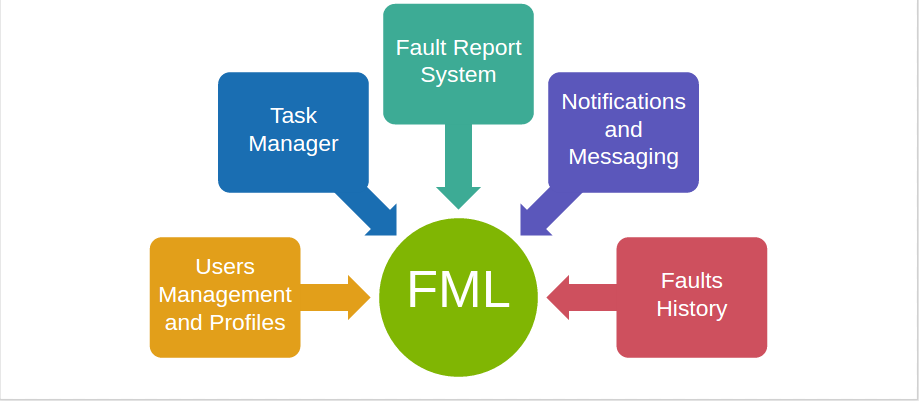
\includegraphics[scale=0.5]{img/subsystems.png}
\caption{Schematic for the subsystems of the project.}
\label{figSubsystems}
\end{figure}

In order to achieve the goals described in chapter \ref{chapIntroduction}, the Fault Manager Lite application is divided into five subsystems: \emph{Task Management}, \emph{Report System}, \emph{Notification and Messaging System}, \emph{User Management} and \emph{Faults History and Statistics}, as seen in figure \ref{figSubsystems}.

A brief description of the functionalities of each mentioned subsystem can be found in the next sections of the document.

\subsection{Task Management}
\label{subsection Task Management}

This subsystem is in charge of the management of repair tasks, which are automatically generated whenever the system receives a new fault report.

Users will use the report system of the application (see \ref{subsection Report System}) to send report faults. These faults will be analyzed by this subsystem and automatically classified depending on their department and priority. Then, their corresponding repair task will be generated based on the form filled by the user and assigned to the closest technician depending on the location of the fault.

Managers will be able to change manually the priority and the person in charge of repairing that fault, which are automatically assigned by the subsystem. The category of the fault can also be modified in case it is not correct; in that case, the fault will then be sent to the manager of the new department. Cleaning department will be treated differently as there is a manager for each building of the UAM campus, so cleaning tasks will be assigned to those managers taking into account this characteristic.

Technicians who have been assigned a repair task will be notified (see \ref{subsection Notification and Messaging System}) and be able to consult the information related to that task. This task information includes: ID of the reporter, location of the fault, timestamp of the report, brief description (subject), detailed description, category, status, priority and occasionally a photography (if any was given by the reporter).

The status of a fault can be: \emph{Pending} (just received by the system, before having been automatically assigned by the system or manually assigned by a manager), \emph{Assigned} (already assigned to a technician, who is or will be eventually solving it) or \emph{Solved} (the task has been successfully completed as the fault has been repaired). Technicians will be able to change the current status of a task assigned to them in order to give managers real-time information about the status of faults' troubleshooting.

Managers will also be able to consult real-time information about repair tasks assigned to members of their departments and make reassignments of tasks in case, for example, of overloading a certain technician or in order to accelerate an specific repair.

\subsection{Report System}
\label{subsection Report System}

This subsystem is in charge of the fault report system, which is the main and most important activity of the whole software system.

Whenever users and/or technicians encounter a fault on the facilities of the campus, they will be able to fill a form in order to report that fault and accelerate its troubleshooting. This fault will then be sent to the FML server, which will assign its repair task to the corresponding technician (see \ref{subsection Task Management}).

The mandatory fields of the form include: a brief description of the problem (subject), a more detailed description (1000 characters maximum length), category (department of the maintenance service) and location (which can be automatically set using GPS technology or manually set by the user in case the GPS function doesn't work properly). The ID of the reporter and the timestamp of the report will be automatically added before sending it.

As an optional field, users can add a photography to their report in case they want to be more specific. The photo will be taken on the fly or added from the user's gallery.

After sending a fault report, the reporter will be able to consult the real-time status of its repair task by selecting that task from his/her fault history (see \ref{subsection Fault History and Statistics}). Reporting a fault enables the opening of a chat conversation with the technician assigned to the repair (see \ref{subsection Notification and Messaging System}).

The report system is also in charge of analyzing newly received fault reports and determine if they can be duplicates of existing reports, by comparing their characteristics: location, similar timestamps and same keywords in the descriptions. Potential duplicates will be sent to the manager, who will decide if they really are the same issue or not.

\subsection{Notification and Messaging System}
\label{subsection Notification and Messaging System}
This subsystem is the one in charge of sending and receiving notifications and messages from the application.

There will exist general and emergency notifications (such as special events in the campus and a fire or blackout in a building, respectively). This notifications will only be sent by managers and all the users will receive that alerts.

Technicians will receive a notification informing them of their assignment of a new task. They will also be able to establish a communication channel (private chat) with the reporter of a fault, in order to ask for more information about that fault. Users will not be able to open this communication channel with the technician in charge of their reported fault, while managers will be able to open a private chat with any member of their departments for a better management and organization of them.

When a fault is repaired and the technician changes its status to solved (see \ref{subsection Task Management}), its reporter will receive a notification about the finish of the repair.

Users and technicians will be able to delete messages or notifications they have received.

\subsection{User Management}
\label{subsection User Management}

This subsystem is in charge of several issues related to the application users, including login, user profile and user's fault history.

In this section, the term `user' will make reference to every member of the UAM that uses the FML application as a reporter or as a member of the maintenance service.

When entering the application, users must introduce their credentials for accessing the UAM's web services. Those credentials will be sent to the UAM members server, which will inform the FML server about the correctness (or not) of them. Login credentials will only be needed once (the first time you access to the application).

Every user will have a profile, including some (optionally filled) information about them. From this profile, every user will have access to their fault report history; every report can be selected in order to see its current status (see \ref{subsection Fault History and Statistics}).

In case of students, this profile will also show them information about their current progress in the achievement of optional credits as a reward for their report history.

This system is also in charge of filtering and/or searching for users in the database. This ability to look for users in the database is only accessible to managers.

\subsection{Fault History and Statistics}
\label{subsection Fault History and Statistics}

This subsystem is in charge of several activities related to fault reports, including their search and the generation of statistics related to them.

When a fault is reported (see \ref{subsection Report System}), that report is saved in the database and its entry can be eventually change. For example, its status will be eventually changed when it gets repaired by a technician, it can be assigned to another technician or its priority can be modified by a manager (see \ref{subsection Task Management}).

Managers will be able to consult the fault database to look for all its entries or apply some filters to look for specific faults. Among the filters that can be applied in the search, there are: category/department, date range, reporter, technician or keyword in the description.

User profiles will make accessible information about fault reports related to those users: reporters will see the faults they have reported and their real-time status, while technicians will see the faults they have repaired or have been assigned to do so. Managers will have all this information available by applying the corresponding filter.

Managers will also be able to generate statistics based on the fault history contained in the database. This statistics can be general, related to their departments or related to a member of their technical staff. The generated statistics can be used to analyze the troubleshooting efficiency of the maintenance service or detect problematic areas.

Users will be able to see a simplified map of the campus with colored signs on it. Each dot represents a reported fault and the color will follow a color code, making its status easily distinguishable depending on it: Pending to assign (red), Assigned (yellow) and Solved (Solved). Only the last 30 reports will be shown in this map at the same time to ensure their visibility.

